\documentclass[border=10pt]{standalone}

\usepackage{tikz}
\usepackage{tikzsymbols}
\usetikzlibrary{calc,patterns,shapes.geometric}

\def\centerarc[#1](#2)(#3:#4:#5){\draw[#1] ($(#2)+({#5*cos(#3)},{#5*sin(#3)})$) arc (#3:#4:#5);}

\begin{document}
	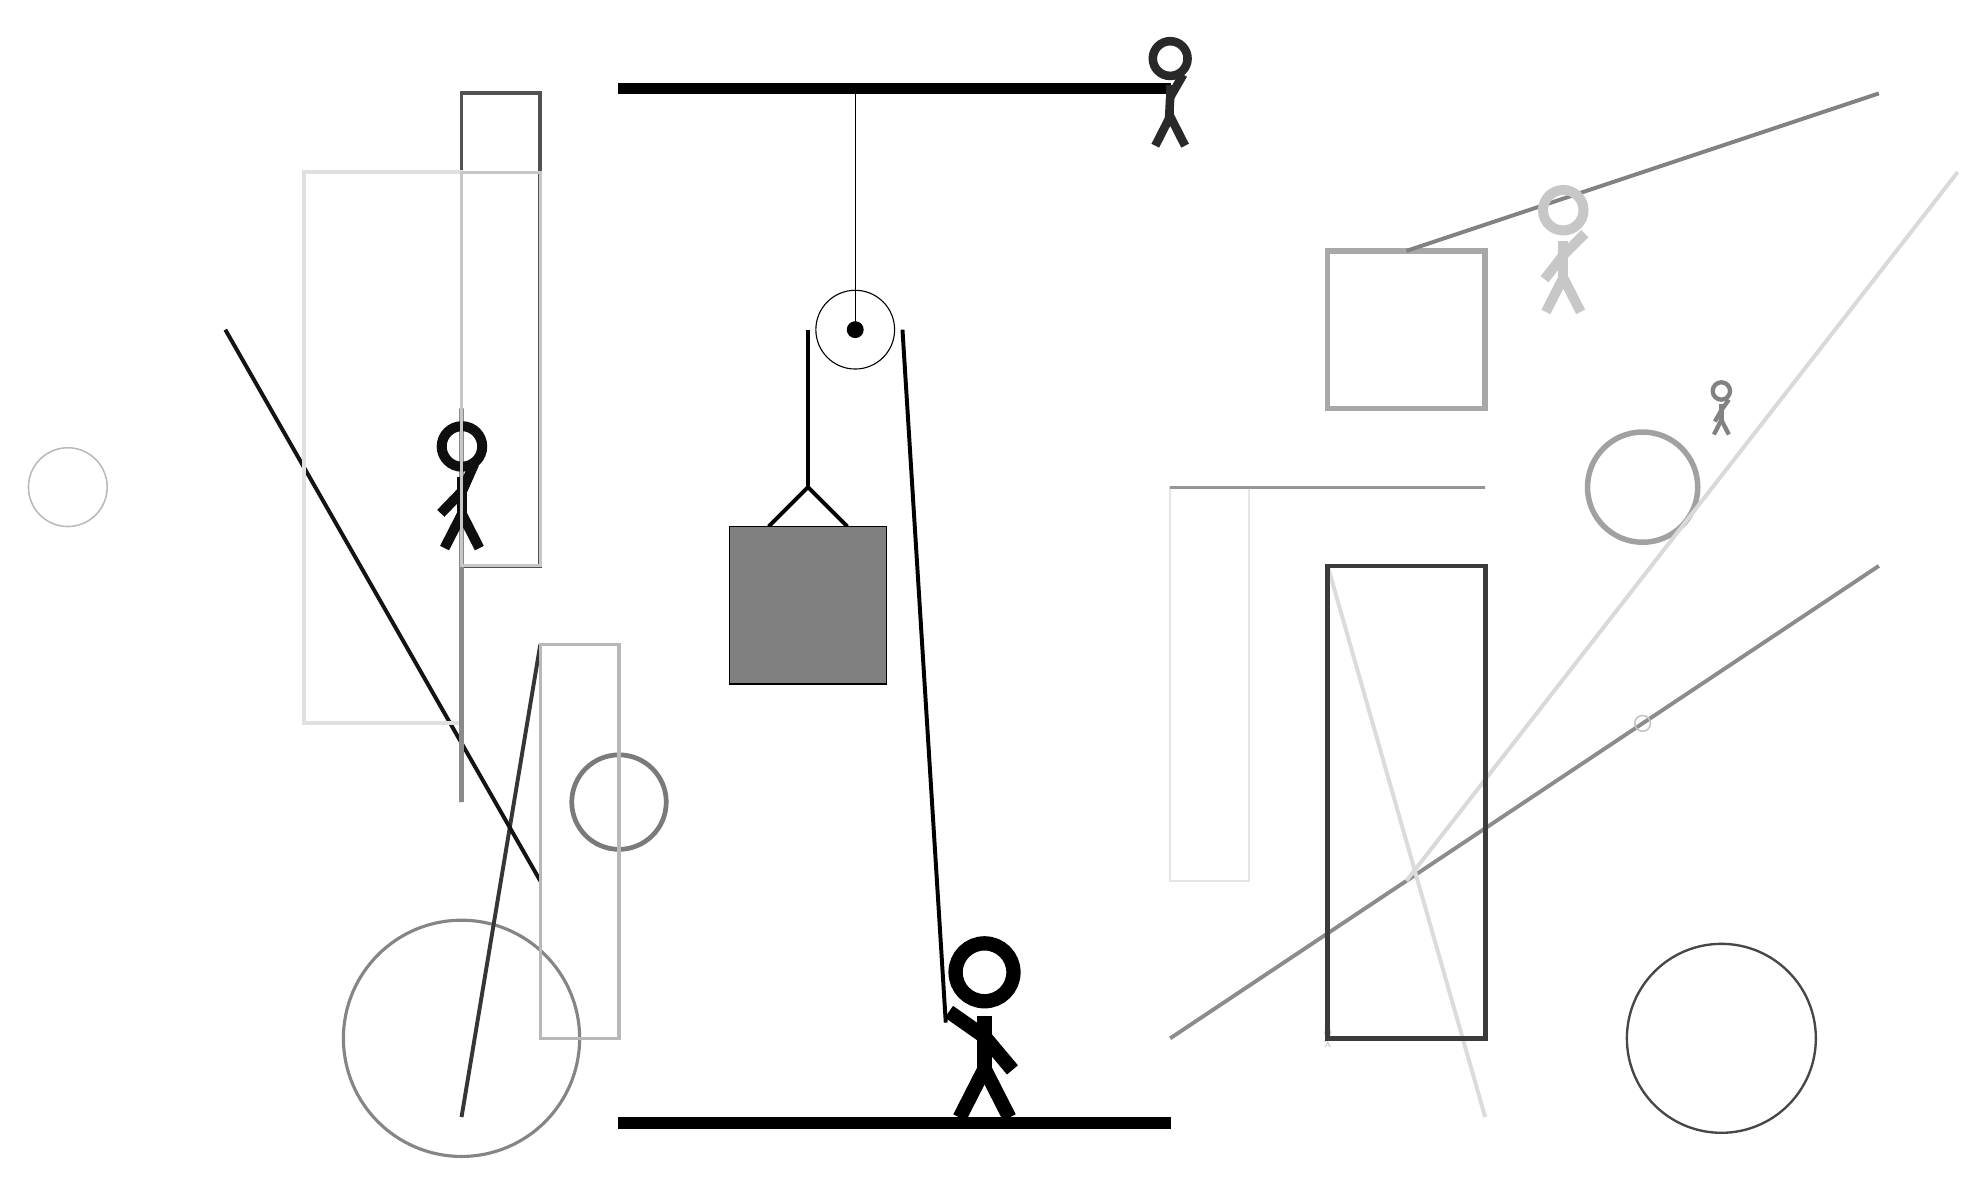
\begin{tikzpicture}
		%%%%% START %%%%%
		
		\draw[fill=black] (-2, 10) rectangle (5, 10.125);
		
		\draw (1, 7) circle (0.5);
		\draw[fill=black] (1, 7) circle (0.1);
		\draw (1, 10) -- (1, 7);
		
		\draw[line width=0.5mm] (-0.1, 4.5) -- (0.4, 5.0) -- (0.9, 4.5);
		\draw[fill=black!50] (-0.6, 4.5) rectangle (1.4, 2.5);
		
		\draw [line width=0.4mm, color=black!48](-4, -2) circle (1.5);
		
		\draw[line width=0.5mm, color=black!79](-4, -3) -- (-3, 3);
		\draw[line width=0.7mm, color=black!34] (7, 6) rectangle (9, 8);
		\draw[line width=0.3mm, color=black!10] (5, 0) rectangle (6, 5);
		
		\node[line width=0.3mm, color=black!18] at (7, -2) {\Strichmaxerl[1][42][45]};
		\draw[line width=0.5mm, color=black!92](-3, 0) -- (-7, 7);
		\draw[line width=0.5mm, color=black!49](8, 8) -- (14, 10);
		\draw [line width=0.7mm, color=black!37](11, 5) circle (0.7);
		\draw[line width=0.5mm, color=black!45](5, -2) -- (14, 4);
		\draw[line width=0.5mm, color=black!68] (-3, 4) rectangle (-4, 10);
		
		\draw [line width=0.6mm, color=black!52](-2, 1) circle (0.6);
		\draw [line width=0.3mm, color=black!72](12, -2) circle (1.2);
		\draw[line width=0.5mm, color=black!12] (-4, 9) rectangle (-6, 2);
		
		\draw[line width=0.5mm, color=black!15](8, 0) -- (15, 9);
		\draw[line width=0.4mm, color=black!41] (5, 5) rectangle (9, 5);
		\draw[line width=0.7mm, color=black!46] (-4, 1) rectangle (-4, 6);
		
		\node[line width=0.4mm, color=black!94] at (-4, 5) {\Strichmaxerl[7][46][66]};
		\draw[line width=0.5mm, color=black!14](9, -3) -- (7, 4);
		\node[line width=0.4mm, color=black!22] at (10, 8) {\Strichmaxerl[7][52][45]};
		\draw[line width=0.4mm, color=black!22] (-4, 4) rectangle (-3, 9);
		\draw[line width=0.6mm, color=black!77] (7, -2) rectangle (9, 4);
		\node[line width=0.7mm, color=black!84] at (5, 10) {\Strichmaxerl[6][87][60]};
		\draw[line width=0.4mm, color=black!28] (-2, 3) rectangle (-3, -2);
		\node[line width=0.2mm, color=black!49] at (12, 6) {\Strichmaxerl[3][60][55]};
		\draw [line width=0.2mm, color=black!27](-9, 5) circle (0.5);
		\draw [line width=0.2mm, color=black!23](11, 2) circle (0.1);
		
		
		\draw[line width=0.5mm] (0.4, 7) -- (0.4, 5.0);
		\centerarc[line width=0.5mm](1, 7)(0:180:0.6);
		\draw[line width=0.5mm](1.6, 7) -- (2.15, -1.8);
		
		\node at (2.6, -1.9) {\Strichmaxerl[10][-35][-50]};
		
		\draw[fill=black] (-2, -3) rectangle (5, -3.15);
		
		%%%%% END %%%%%
	\end{tikzpicture}
\end{document}